The electroweak process \Wgstar~ contributes as background to the Higgs signal in the case one of the 
three leptons in the final state is not properly detected. 
We can consider separately the two cases where the lepton pair from the \Astar are electrons
or muons. The cross section for the \ensuremath{l^{\pm}e^{+}e^{-}} final state
(with \ensuremath{l^{\pm}}=\ensuremath{\mu^{\pm}} or \ensuremath{e^{\pm}} being the lepton from the \W decay) 
is larger by a factor $\sim3$ with respect to the \ensuremath{l^{\pm}\mu^{+}\mu^{-}} case
due to the lower production threshold 
(defined by \ensuremath{2M_{l}}) and the steep rising of \ensuremath{d\sigma/dM_{\gamma}}.
The leptons originated from the virtual photon feature small opening angle and small invariant mass.
At least one of the two leptons is soft with an average \pt~ of $\sim5$ GeV.
In the \ensuremath{l^{\pm}e^{+}e^{-}} case the way of faking the signal is similarly to the \wgamma background 
when the photon converts in the material close to the interaction vertex 
(it can be seen as a sort of ``prompt'' conversion). 
For the \ensuremath{l^{\pm}\mu^{+}\mu^{-}} final state, the low \pt~ of the softest muon often prevents
it to reach the muon stations and thus to be identified as a muon.

We have at disposal a leading order matrix element based Monte Carlo (Madgraph) simulation
of the \Wgstar~ whose normalization needs however to be estimated from data.
To achieve that a cross section-like measurement has been performed 
aimed at isolating this process in the data.
Given the large overwhelming background we should deal with for the \ensuremath{l^{\pm}e^{+}e^{-}} 
case, we focused only on the \ensuremath{l^{\pm}\mu^{+}\mu^{-}} final state.
The \Wgstar~ control region has been defined such to reach high purity. 
The following selections have been applied:
\begin{itemize}
\item the muon pair associated to the virtual photon needs to have opposite charge. In the case of
\ensuremath{\mu\mu\mu} final state, the pair with lowest mass is assumed to originate from the \Astar.
\item the muon isolation is redefined not to consider the other muon in the case it is closer than \delR=0.3.
\item events with less than 2 jets are considered, anti b-tagging is required for all jets with \ensuremath{p_\mathrm{T}>10} GeV.
\item minMet$>20$, \mt$>20$ (where \mt is computed from the \W's lepton and the \met).
\item \ensuremath{M_{\mu\mu}<12} GeV.
\end{itemize} 

These cuts are meant to suppress mainly top and QCD induced background.
The upper bound on the di-muon mass is set to get ride of the interference between
\Wgstar~ and \ensuremath{\W\Astar}. 
The Monte Carlo used for the latter includes in fact both \Astar and \Zstar contributions
and takes properly into account the interference between them.
The plot in Figure \ref{fig:WgammaStarMass} compares the 
mass distributions of the muon pair associated with the virtual photon for data and Monte Carlo
once all the selections listed above are applied but \ensuremath{M_{\mu\mu}<12} GeV.
The data correspond to an integrated luminosity equal to 4\ifb.

\begin{figure}[hbt]
\begin{center}
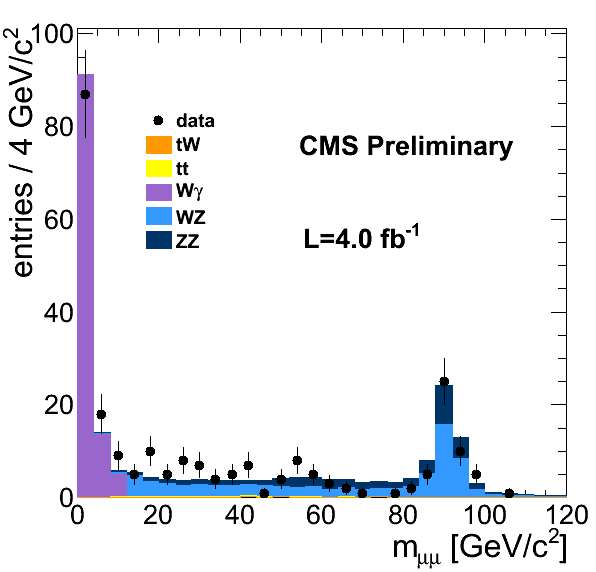
\includegraphics[width=0.5\linewidth]{figures/WGammaStar_mass_wholeSpectrum.png} 
\caption{\label{fig:WgammaStarMass}\protect Comparison of data and Monte Carlo for  
mass distributions of the muon pair associated with the virtual photon. 
All the selections defining the \Wgstar~ control region are applied but \ensuremath{M_{\mu\mu}<12} GeV.}
\end{center}
\end{figure}

The plots in Figure \ref{fig:WgammaStar}, displaying data and MC distributions for
the muon pair associated with the virtual photon, 
(left: opening angle, center: di-muon mass, right: \pt~ of the softest muon) 
assess the compatibility of the data belonging
to the control region with the expectations from the \Wgstar~ Monte Carlo.
The small differences between the data and MC shapes can be explained by the mismodeling
in the Monte Carlo of the reconstruction efficiencies for very soft leptons 
(scale factors to match the data trigger and reconstruction efficiencies very computed
for leptons only down to 10 GeV).
The contribution for top background result to be negligible.
As a further cross check, we estimated the data yields for events satisfying the \Wgstar~ selections
but with the muons with smallest invariant mass having the same sign. 
Contrary to \Wgstar, QCD and top backgrounds have in fact about the same chance to produce 
same sign and opposite muons. Only four data counts are found the mass region relevant for 
the \Wgstar~ process (\ensuremath{M_{\mu^{\pm}\mu^{\pm}}<12} GeV), 
confirming thus that the contamination from processes different than \Wgstar~ is very limited.


\begin{figure}[hbt]
\begin{center}
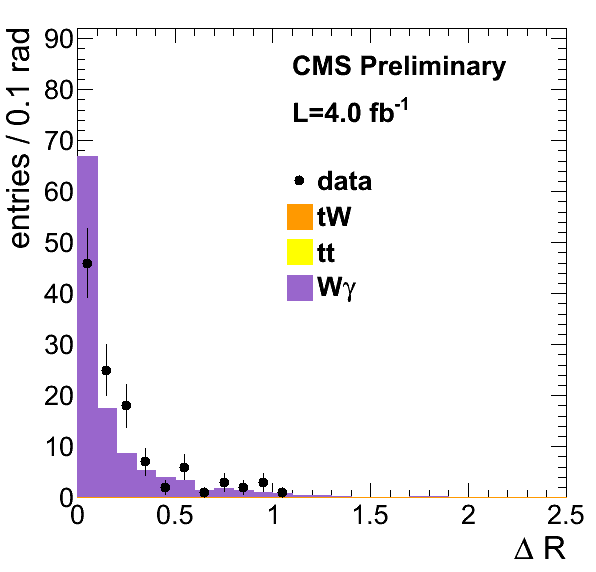
\includegraphics[width=0.3\linewidth]{figures/WGammaStar_dR.png} 
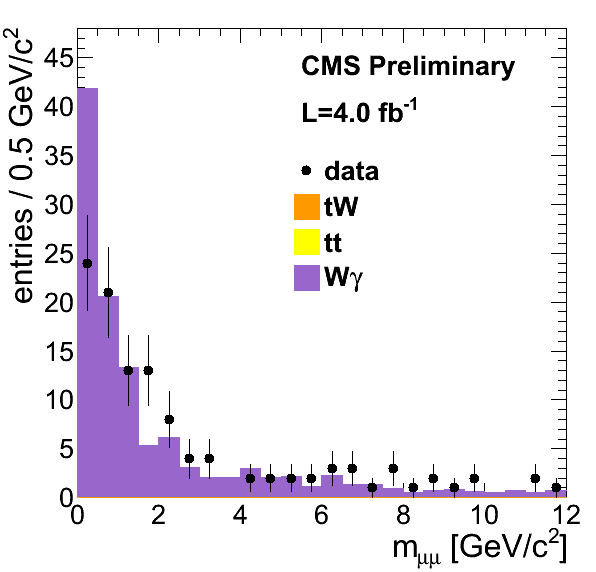
\includegraphics[width=0.3\linewidth]{figures/WGammaStar_mass.png}
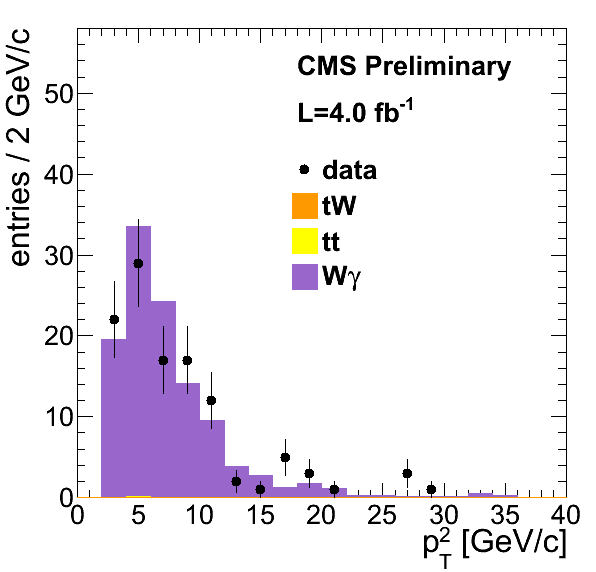
\includegraphics[width=0.3\linewidth]{figures/WGammaStar_3rdLep.png}
\caption{\label{fig:WgammaStar}\protect Comparison of data and Monte Carlo for three 
main distributions of the muons associated with the virtual photon in the \Wgstar~ control region. 
Left: opening angle (\delR).
Center: di-muon mass.
Right:. softest muon \pt.}
\end{center}
\end{figure}

Table \ref{tab:wgamma} summarizes the results of the \Wgstar~ measurement and the
normalization of the corresponding Monte Carlo. As already discussed, the background
contamination turned out to be almost negligible.
The data yields correspond to \ensuremath{L=4\ifb}.
The not so large difference from unity of the overall {\em k-}factor,
is giving further confidence on the accuracy of the Monte Carlo simulation.
The same {\em k-}factor is used hereafter for the other two relevant final states
where the virtual photon decays to an electron pair.
Once normalized one data as just described, the Madgraph MC is used to predict the yields
after the standard Higgs selection.

\begin{table}
\begin{center}
\begin{tabular}{|c|c|c|c|}
\hline
& \ensuremath{e\mu\mu} & \ensuremath{\mu\mu\mu} & \ensuremath{\mu\mu} \\
\hline
data yields & 26 & 88 & 114 \\
\hline
top background & 0 & 0.2 & 0.2 \\
\hline
background from SS & 0 & 4 & 4 \\ 
\hline
(raw) \Wgstar~ MC yields & $20\pm1.1$ & $52\pm1.7$ & $72\pm2.0$ \\
\hline
\hline
{\em k-}factor & $1.3\pm0.25$ & $1.7\pm0.2$ & $1.53\pm0.15$ \\
\hline

\end{tabular}
\caption{Results of the measurements in the \Wgstar control region.
{\em k-}factors are computed as ratios between the data yields and the MC predictions.
Results are shown separately for \ensuremath{e\mu\mu} and \ensuremath{\mu\mu\mu} final states
in the first two columns, whereas the third one consider them together.
The data yields correspond to \ensuremath{L=4\ifb}. 
\label{tab:wgamma}}
\end{center}
\end{table}

